\section{System}
\label{sec:system}

\subsection{Acoustic model}

We start from the baseline's strongest balanced checkpoint: XLS-R-300M
\cite{babu2022xlsr}, a multilingual wav2vec~2.0 model
\cite{baevski2020wav2vec2} of 315M parameters, continued pre-training on 65 hours of
unlabelled Puno Quechua audio, then CTC fine-tuning \cite{graves2006ctc} on
validated and silver data. Continued pre-training is what adapts a multilingual
model to the phonology of a language it has barely seen, and is reliably worth
its cost in low-resource settings \cite{dehaven2022cpt,getman2024adaptation};
we reuse the authors' checkpoint rather than replicate it.

The released checkpoints are fairseq files, and fairseq 0.12.2 has no wheel for
current Python versions, so we port the weights to the HuggingFace
\texttt{Wav2Vec2ForCTC} implementation \cite{wolf2020transformers}.
As a correctness check, the converted model scores 27.26 WER on the baseline's
out-of-domain set against its published 27.4, confirming the port is faithful.

Fine-tuning runs for 500 updates at learning rate $2\times10^{-5}$
(Section~\ref{sec:plateau}). Batches are formed by total audio duration rather
than clip count: clips range from under two seconds to thirty, so any fixed
count either exhausts memory on long clips or wastes the device on short ones.


\begin{figure}[tb]
\centering
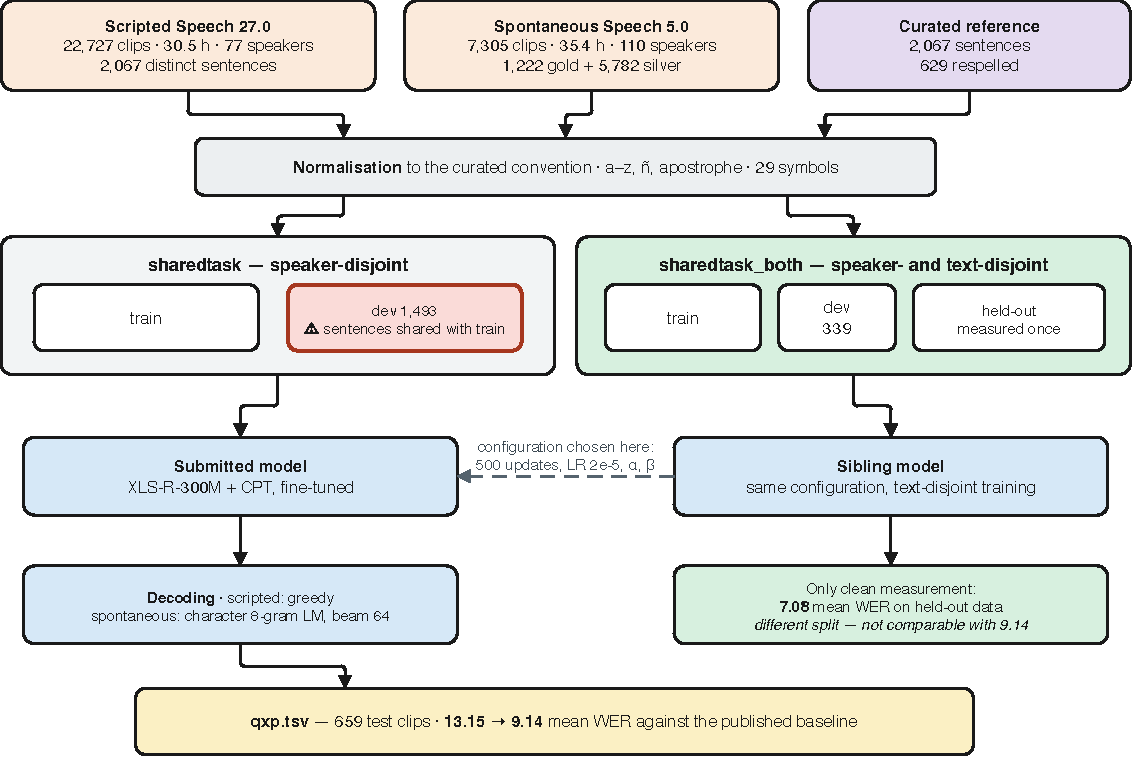
\includegraphics[width=\textwidth]{figures/pipeline_pastel.pdf}
\caption{Data, splits and system. Two splits are built from the same
normalised corpora. The submitted model trains on \texttt{sharedtask}, whose
development sentences also occur in training; its sibling trains on
\texttt{sharedtask\_both}, which shares neither speakers nor sentences and so
yields the only measurement free of overlap. The dashed arrow marks what
passes between them: the configuration is chosen on the sibling and applied to the
submitted model, not its weights.}
\label{fig:pipeline}
\end{figure}

\subsection{Decoding}

Spontaneous speech is decoded with a language model over characters rather
than words; Section~\ref{sec:discussion} explains why. These language models
are character $n$-grams estimated by counting, with modified
Kneser-Ney smoothing \cite{chen1996smoothing} to reserve probability for
sequences the training text never shows. We check each one against KenLM
\cite{heafield2011kenlm}: a distribution must sum to one, so for 200 contexts
we sum the probability of every possible next character; the largest deviation
was of order $10^{-6}$.

Decoding uses flashlight-text's \emph{lexicon-free} beam search
\cite{kahn2022flashlight} with beam width 64. The qualifier matters: a
conventional decoder consults the language model only when a word ends, against
a fixed vocabulary, which a character model cannot use. A lexicon-free decoder
scores it on every character as it is emitted. A hypothesis scores
\begin{equation}
\sum \log p_{\text{CTC}}
\;+\; \alpha \sum \log P_{\text{LM}}
\;+\; \beta\,n_{\text{words}},
\label{eq:score}
\end{equation}
where $\alpha$ weights the language model against the acoustics and $\beta$
offsets its preference for shorter word sequences.

The final configuration decodes scripted speech greedily and spontaneous speech
with an order-8 model trained on gold and silver spontaneous text,
$\alpha = 0.5$, $\beta = 0$. Section~\ref{sec:lmneg} explains why scripted
speech ends up with no language model at all.
